\documentclass[a4paper,11pt]{report}
\usepackage[T1]{fontenc}
\usepackage[utf8]{inputenc}
\usepackage{lmodern}
\usepackage{booktabs}
\usepackage[margin=3.5cm]{geometry}
\usepackage{color, colortbl}
\usepackage{graphicx}
\usepackage[binary-units=true]{siunitx}  
\usepackage[cmex10]{amsmath}

\parindent=0mm
\parskip=3mm

\definecolor{Gray}{gray}{0.9}

\title{MiloSAR Documentation \\ \vspace{0.5cm} \Large Version 0.2}
\author{Darryn Jordan}

\begin{document}

\maketitle
\tableofcontents

\chapter{Introduction}

\chapter{Synthesizer}

\section{$ \mu $Wire Interface}

The LMX2492EVM is packaged with a USBtoMANY converter, enabling users to program the evaluation module through its $ \mu $Wire connector using TI's CodeLoader. This process is however tedious, especially when programming two synthesizers with different waveforms. The LMX2492 datasheet provides the timing requirements and clocking structure for programming the synthesizer through its $ \mu $Wire connector pins. GPIO pins on the Red Pitaya were used to program both synthesizers efficiently. Figure~\ref{fig:rp_synth_connect} illustrates the connection between the Red Pitaya and two LMX2492 evaluation boards.
\begin{figure}[h!]
    \begin{center}
        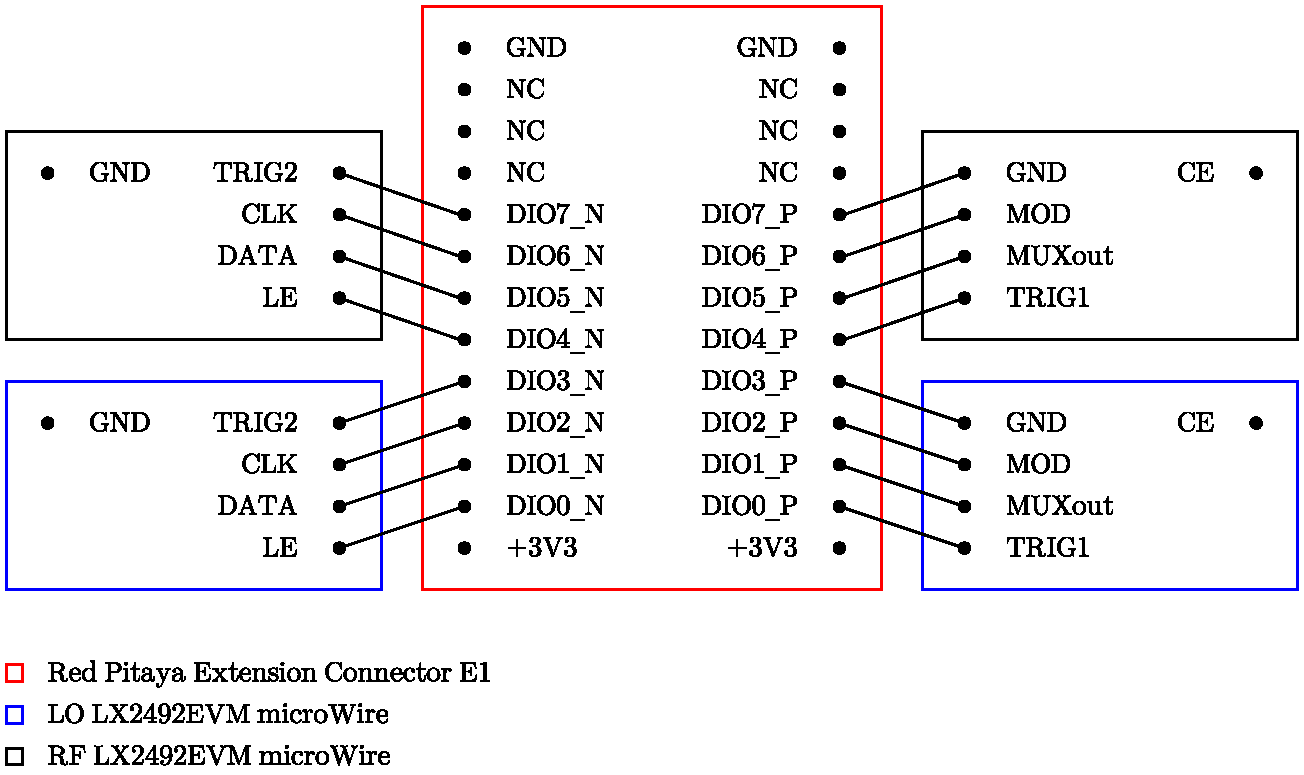
\includegraphics[width=\textwidth]{images/rp_synth_connections.pdf}
        \caption{Wiring diagram for connection between Red Pitaya and the LMX2492.}
        \label{fig:rp_synth_connect}
    \end{center}
\end{figure}

\chapter{FPGA}

\section{Registers}

% \subsection{Configuration}
% The configuration register is currently only used to set the decimation factor for reducing sampling rate. Sixteen bits are reserved for later use.
% \begin{table}[ht]
%     \caption{General configuration register.}
%     \begin{center}
%         \begin{tabular}{|c|c|c|c|c|c|c|c|c|c|c|c|c|c|c|c|}
%             \hline
%             \rowcolor{Gray}
%             \multicolumn{8}{|c|}{B3} & \multicolumn{8}{c|}{B2}\\
%             \hline
%             31 & 30 & 29 & 28 & 27 & 26 & 25 & 24 & 23 & 22 & 21 & 20 & 19 & 18 & 17 & 16 \\
%             \hline
%             \multicolumn{8}{|c|}{Reserved [31:24]} & \multicolumn{8}{c|}{Reserved [23:16]}\\
%             \hline  
%             
%             \addlinespace[0.5cm]
%             
%             \hline 
%             \rowcolor{Gray}
%             \multicolumn{8}{|c|}{B1} & \multicolumn{8}{c|}{B0}\\
%             \hline
%             15 & 14 & 13 & 12 & 11 & 10 & 9 & 8 & 7 & 6 & 5 & 4 & 3 & 2 & 1 & 0 \\
%             \hline
%             \multicolumn{16}{|c|}{Decimation Factor [15:0]}\\
%             \hline
%         \end{tabular}
%     \end{center}
%     \label{tab:config_reg}
% \end{table}
% \newpage

\subsection{Channel X Status}
Both recording channels within the FPGA require a status register to provide the CPU with the location of the RAM writer's current pointer location.
\begin{table}[ht]
    \caption{Channel X status register.}
    \begin{center}
        \begin{tabular}{|c|c|c|c|c|c|c|c|c|c|c|c|c|c|c|c|}
            \hline
            \rowcolor{Gray}
            \multicolumn{8}{|c|}{B3} & \multicolumn{8}{c|}{B2}\\
            \hline
            31 & 30 & 29 & 28 & 27 & 26 & 25 & 24 & 23 & 22 & 21 & 20 & 19 & 18 & 17 & 16 \\
            \hline
            \multicolumn{16}{|c|}{Channel X Pointer [31:16]}\\
            \hline  
            
            \addlinespace[0.5cm]
            
            \hline 
            \rowcolor{Gray}
            \multicolumn{8}{|c|}{B1} & \multicolumn{8}{c|}{B0}\\
            \hline
            15 & 14 & 13 & 12 & 11 & 10 & 9 & 8 & 7 & 6 & 5 & 4 & 3 & 2 & 1 & 0 \\
            \hline
            \multicolumn{16}{|c|}{Channel X Pointer [15:0]}\\
            \hline
        \end{tabular}
    \end{center}
    \label{tab:status_reg}
\end{table}
\newpage

\subsection{GPIO}
The GPIO register is currently haphazard and contains the clock divisor value, which is used to set the PRF. Furthermore, an enable flag, bit 8, is used to enable the receive chain. It is suggested that both of these settings be moved the the configuration register once the decimation factor is fixed. 
\begin{table}[ht]
    \caption{GPIO register.}
    \begin{center}
        \begin{tabular}{|c|c|c|c|c|c|c|c|c|c|c|c|c|c|c|c|}
            \hline
            \rowcolor{Gray}
            \multicolumn{8}{|c|}{B3} & \multicolumn{8}{c|}{B2}\\
            \hline
            31 & 30 & 29 & 28 & 27 & 26 & 25 & 24 & 23 & 22 & 21 & 20 & 19 & 18 & 17 & 16 \\
            \hline
            \multicolumn{16}{|c|}{Clock Divisor [31:16]}\\
            \hline  
            
            \addlinespace[0.5cm]
            
            \hline 
            \rowcolor{Gray}
            \multicolumn{8}{|c|}{B1} & \multicolumn{8}{c|}{B0}\\
            \hline
            15 & 14 & 13 & 12 & 11 & 10 & 9 & 8 & 7 & 6 & 5 & 4 & 3 & 2 & 1 & 0 \\
            \hline
            \multicolumn{7}{|c|}{Clock Divisor [15:9]} & E & \multicolumn{8}{c|}{GPION [7:0]}\\
            \hline
        \end{tabular}
    \end{center}
    \label{tab:gpio_reg}
\end{table}
\newpage

\subsection{Reference Signal Phase Increment}
Provides the FPGA with the DDS phase increment used to generate the \SI{50}{\MHz} phase reference signal.
\begin{table}[ht]
    \caption{Synthesizer reference signal phase increment register.}
    \begin{center}
        \begin{tabular}{|c|c|c|c|c|c|c|c|c|c|c|c|c|c|c|c|}
            \hline
            \rowcolor{Gray}
            \multicolumn{8}{|c|}{B3} & \multicolumn{8}{c|}{B2}\\
            \hline
            31 & 30 & 29 & 28 & 27 & 26 & 25 & 24 & 23 & 22 & 21 & 20 & 19 & 18 & 17 & 16 \\
            \hline
            \multicolumn{16}{|c|}{Phase Increment [31:16]}\\
            \hline  
            
            \addlinespace[0.5cm]
            
            \hline 
            \rowcolor{Gray}
            \multicolumn{8}{|c|}{B1} & \multicolumn{8}{c|}{B0}\\
            \hline
            15 & 14 & 13 & 12 & 11 & 10 & 9 & 8 & 7 & 6 & 5 & 4 & 3 & 2 & 1 & 0 \\
            \hline
            \multicolumn{16}{|c|}{Phase Increment [15:0]}\\
            \hline
        \end{tabular}
    \end{center}
    \label{tab:ref_phase_inc}
\end{table}
\newpage

\subsection{Cancellation Signal Phase Increment}
Provides the FPGA with the DDS phase increment used to generate the IF cancellation signal.
\begin{table}[ht]
    \caption{Cancellation signal phase increment register.}
    \begin{center}
        \begin{tabular}{|c|c|c|c|c|c|c|c|c|c|c|c|c|c|c|c|}
            \hline
            \rowcolor{Gray}
            \multicolumn{8}{|c|}{B3} & \multicolumn{8}{c|}{B2}\\
            \hline
            31 & 30 & 29 & 28 & 27 & 26 & 25 & 24 & 23 & 22 & 21 & 20 & 19 & 18 & 17 & 16 \\
            \hline
            \multicolumn{16}{|c|}{Phase Increment [31:16]}\\
            \hline  
            
            \addlinespace[0.5cm]
            
            \hline 
            \rowcolor{Gray}
            \multicolumn{8}{|c|}{B1} & \multicolumn{8}{c|}{B0}\\
            \hline
            15 & 14 & 13 & 12 & 11 & 10 & 9 & 8 & 7 & 6 & 5 & 4 & 3 & 2 & 1 & 0 \\
            \hline
            \multicolumn{16}{|c|}{Phase Increment [15:0]}\\
            \hline
        \end{tabular}
    \end{center}
    \label{tab:canc_phase_inc}
\end{table}

\subsection{Cancellation Signal Phase Offset}
Provides the FPGA with the DDS phase offset used to adjust the phase of the cancellation signal.
\begin{table}[ht]
    \caption{Cancellation signal phase offset register.}
    \begin{center}
        \begin{tabular}{|c|c|c|c|c|c|c|c|c|c|c|c|c|c|c|c|}
            \hline
            \rowcolor{Gray}
            \multicolumn{8}{|c|}{B3} & \multicolumn{8}{c|}{B2}\\
            \hline
            31 & 30 & 29 & 28 & 27 & 26 & 25 & 24 & 23 & 22 & 21 & 20 & 19 & 18 & 17 & 16 \\
            \hline
            \multicolumn{16}{|c|}{Phase Offset [31:16]}\\
            \hline  
            
            \addlinespace[0.5cm]
            
            \hline 
            \rowcolor{Gray}
            \multicolumn{8}{|c|}{B1} & \multicolumn{8}{c|}{B0}\\
            \hline
            15 & 14 & 13 & 12 & 11 & 10 & 9 & 8 & 7 & 6 & 5 & 4 & 3 & 2 & 1 & 0 \\
            \hline
            \multicolumn{16}{|c|}{Phase Offset [15:0]}\\
            \hline
        \end{tabular}
    \end{center}
    \label{tab:canc_phase_off}
\end{table}
\newpage

\subsection{Profile Integrator Configuration}
Specify the number of samples to integrate over and the number of pulses to integrate. Number of samples is currently limited to \SI{13}{\bit}s. This can be increased to \SI{15}{\bit}s if the FIFO depth is increased in the FPGA design. 
\begin{table}[ht]
    \caption{Cancellation signal phase offset register.}
    \begin{center}
        \begin{tabular}{|c|c|c|c|c|c|c|c|c|c|c|c|c|c|c|c|}
            \hline
            \rowcolor{Gray}
            \multicolumn{8}{|c|}{B3} & \multicolumn{8}{c|}{B2}\\
            \hline
            31 & 30 & 29 & 28 & 27 & 26 & 25 & 24 & 23 & 22 & 21 & 20 & 19 & 18 & 17 & 16 \\
            \hline
            \multicolumn{16}{|c|}{Number of Pulses [31:16]}\\
            \hline  
            
            \addlinespace[0.5cm]
            
            \hline 
            \rowcolor{Gray}
            \multicolumn{8}{|c|}{B1} & \multicolumn{8}{c|}{B0}\\
            \hline
            15 & 14 & 13 & 12 & 11 & 10 & 9 & 8 & 7 & 6 & 5 & 4 & 3 & 2 & 1 & 0 \\
            \hline
            \multicolumn{3}{|c|}{Reserved} & \multicolumn{13}{c|}{Number of Samples [12:0]}\\
            \hline
        \end{tabular}
    \end{center}
    \label{tab:prof_int_config}
\end{table}

\subsection{Profile Integrator Index}
Specify the start and end index of the integrated profile. \textbf{Note that sample indexing begins at one}.
\begin{table}[ht]
    \caption{Profile integrator index register.}
    \begin{center}
        \begin{tabular}{|c|c|c|c|c|c|c|c|c|c|c|c|c|c|c|c|}
            \hline
            \rowcolor{Gray}
            \multicolumn{8}{|c|}{B3} & \multicolumn{8}{c|}{B2}\\
            \hline
            31 & 30 & 29 & 28 & 27 & 26 & 25 & 24 & 23 & 22 & 21 & 20 & 19 & 18 & 17 & 16 \\
            \hline
            \multicolumn{16}{|c|}{End Index [31:16]}\\
            \hline  
            
            \addlinespace[0.5cm]
            
            \hline 
            \rowcolor{Gray}
            \multicolumn{8}{|c|}{B1} & \multicolumn{8}{c|}{B0}\\
            \hline
            15 & 14 & 13 & 12 & 11 & 10 & 9 & 8 & 7 & 6 & 5 & 4 & 3 & 2 & 1 & 0 \\
            \hline
            \multicolumn{16}{|c|}{Start Index [15:0]}\\
            \hline
        \end{tabular}
    \end{center}
    \label{tab:prof_index_config}
\end{table}
\newpage

\section{Digital Receiver Design}
Design of the digital receiver begins with the selection of a suitable analogue bandpass filter. The SBP-10.7+ bandpass filter (BPF), procured from Mini-Circuits, features a \SI{3}{\dB} bandwidth of \SI{3.8}{MHz} and lower-side cut-off frequency, $ f_{\SI{3}{\dB}} $, of \SI{8.5}{\dB} as illustrated in Figure~\ref{fig:band_pass_response}. The SBP-10.7+ serves a dual role in suppressing feed-through and implementing sensitivity frequency-control. 
\begin{figure}[h!]
    \begin{center}
        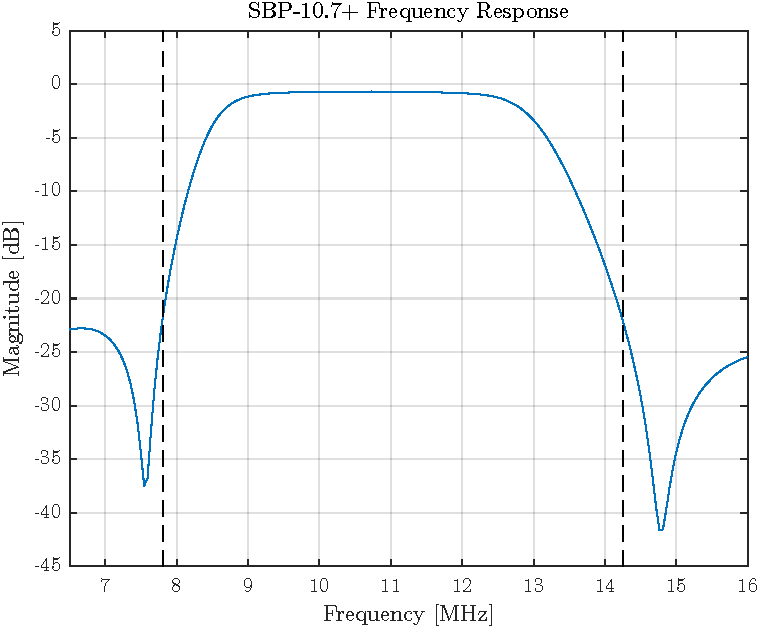
\includegraphics[width=\textwidth]{images/band_pass_response}
        \caption{Frequency response of the SBP-10.7+ BPF with dashed lines indicating the Nyquist band of interest.}
        \label{fig:band_pass_response}
    \end{center}
\end{figure}

Following the SBP-10.7+, the beat spectrum is oversampled at a rate of \SI{125}{\MHz} using the Red Pitaya. This results in a spreading of quantization noise over the full sampled bandwidth (\SI{62.5}{\MHz}). With appropriate filtering, quantization noise is greatly reduced. An additional benefit of oversampling is the ability to perform decimation through averaging in order to increase the effective number of bits (ENOB). Equation~\ref{eqn:oversampling} reveals that an additional \SI{1.5}{\bit}s are gained through decimation by a factor of 8.
\begin{align} \label{eqn:oversampling}
n = \log_4 (DF)
\end{align}
The SBP-10.7+ BPF is ideally positioned to make use of the second Nyquist zone when using a decimation factor (DF) of 8. All signals of interest must therefore be contained within the $ f_{s}/2 $ to $ f_{s} $ band, or \SI{7.8125}{\MHz} to \SI{15.625}{\MHz} respectively, illustrated by the dashed lines in Figure~\ref{fig:band_pass_response}. Components out of the Nyquist band of interest are therefore attenuated by more than \SI{20}{\dB}. 

Having oversampled the beat spectrum at IF, the first step in the digital receive chain is pass the signal through the bandpass FIR decimation filter illustrated in Figure~\ref{fig:fir_filter}.  
\begin{figure}[h!]
    \begin{center}
        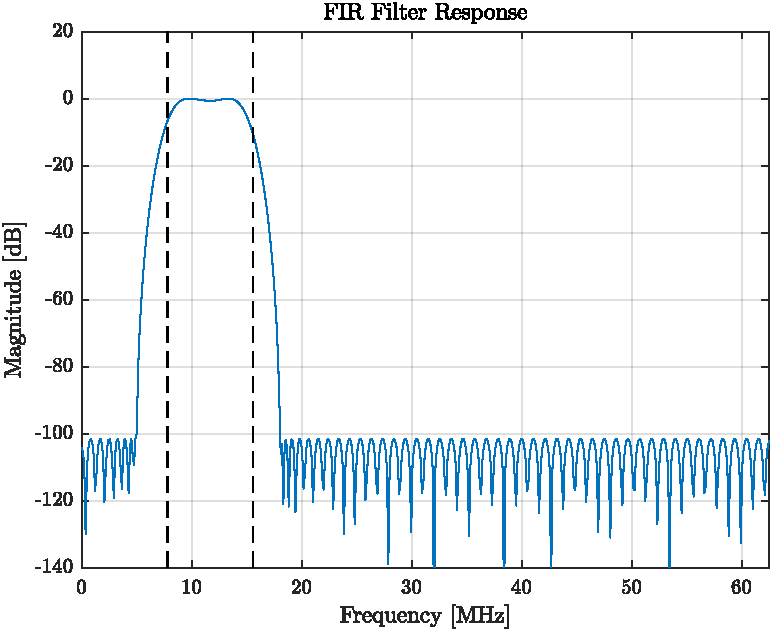
\includegraphics[width=\textwidth]{images/fir_filter}
        \caption{Frequency response of the FIR filter within the Red Pitaya.}
        \label{fig:fir_filter}
    \end{center}
\end{figure}

It is important to note that the SBP-10.7+ analogue filter suppresses signals out of the second Nyquist band by an additional \SI{20}{\dB}. Over \SI{100}{\dB} of suppression is provided by this 115-tap FIR filter. In addition to this, the filter is responsible for implementing decimation through averaging. As explained previously, \SI{1.5}{\bit}s are gained through averaging. The output samples are however limited to \SI{15}{\bit} samples, taking advantage of an extra \SI{1}{\bit}.

Both the main and reference channel pass through these filters and are saved to disk for further processing in Matlab. Figure~\ref{fig:aliased_down_conversion} illustrates the frequency domain steps for demodulating the main channel using the reference channel.

The topmost two spectrums illustrate the process of Nyquist folding during undersampling. The analogue beat spectrum folds around $ f_{s}/2 $, resulting in a flipped digital replica of the spectrum. The third spectrum is simply the same result of Nyquist folding for the reference channel. 
\begin{figure}[h!]
    \begin{center}
        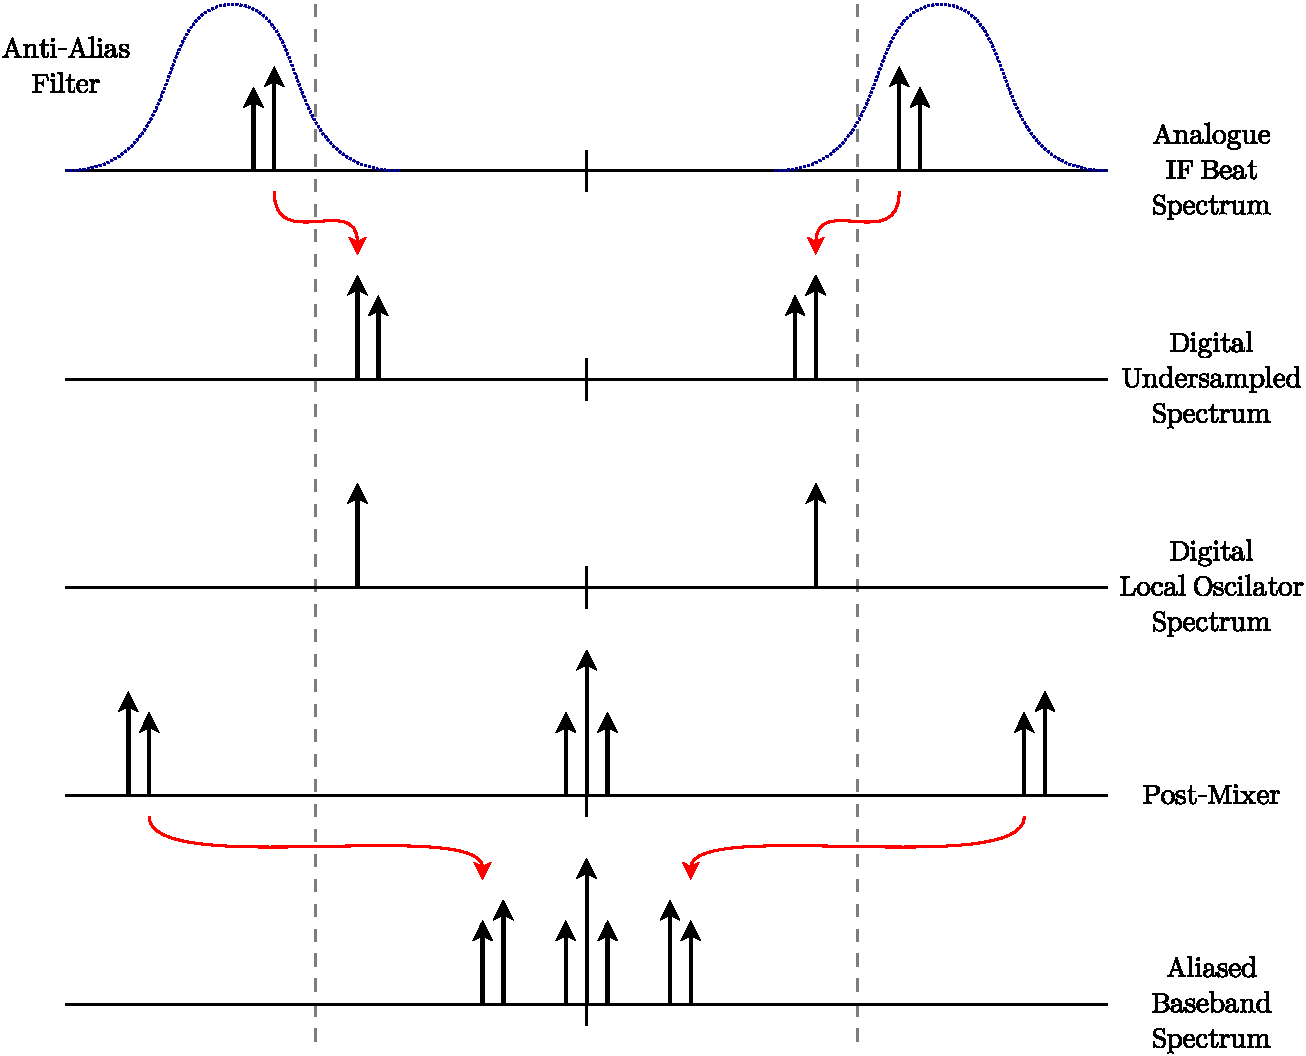
\includegraphics[width=\textwidth]{images/aliased_down_conversion}
        \caption{Down-conversion with aliasing owing to low sample rate.}
        \label{fig:aliased_down_conversion}
    \end{center}
\end{figure}

The digitised main and reference channels are then multiplied together to perform demodulation, however, the post-mixer spectrum reveals a potential problem. The components shifted to a higher frequency fall out to the sampled bandwidth and therefore fold into the baseband spectrum. This unforeseen problem can however be avoided by zeroing the components that fold into the baseband spectrum before mixing.

\newpage
Figure~\ref{fig:anti_alias_down_conversion} illustrates the result of nullifying half of the main and reference channel before mixing. This process can be seen to prevent aliasing and avoid a doubling of the DC component.
\begin{figure}[!ht]
    \begin{center}
        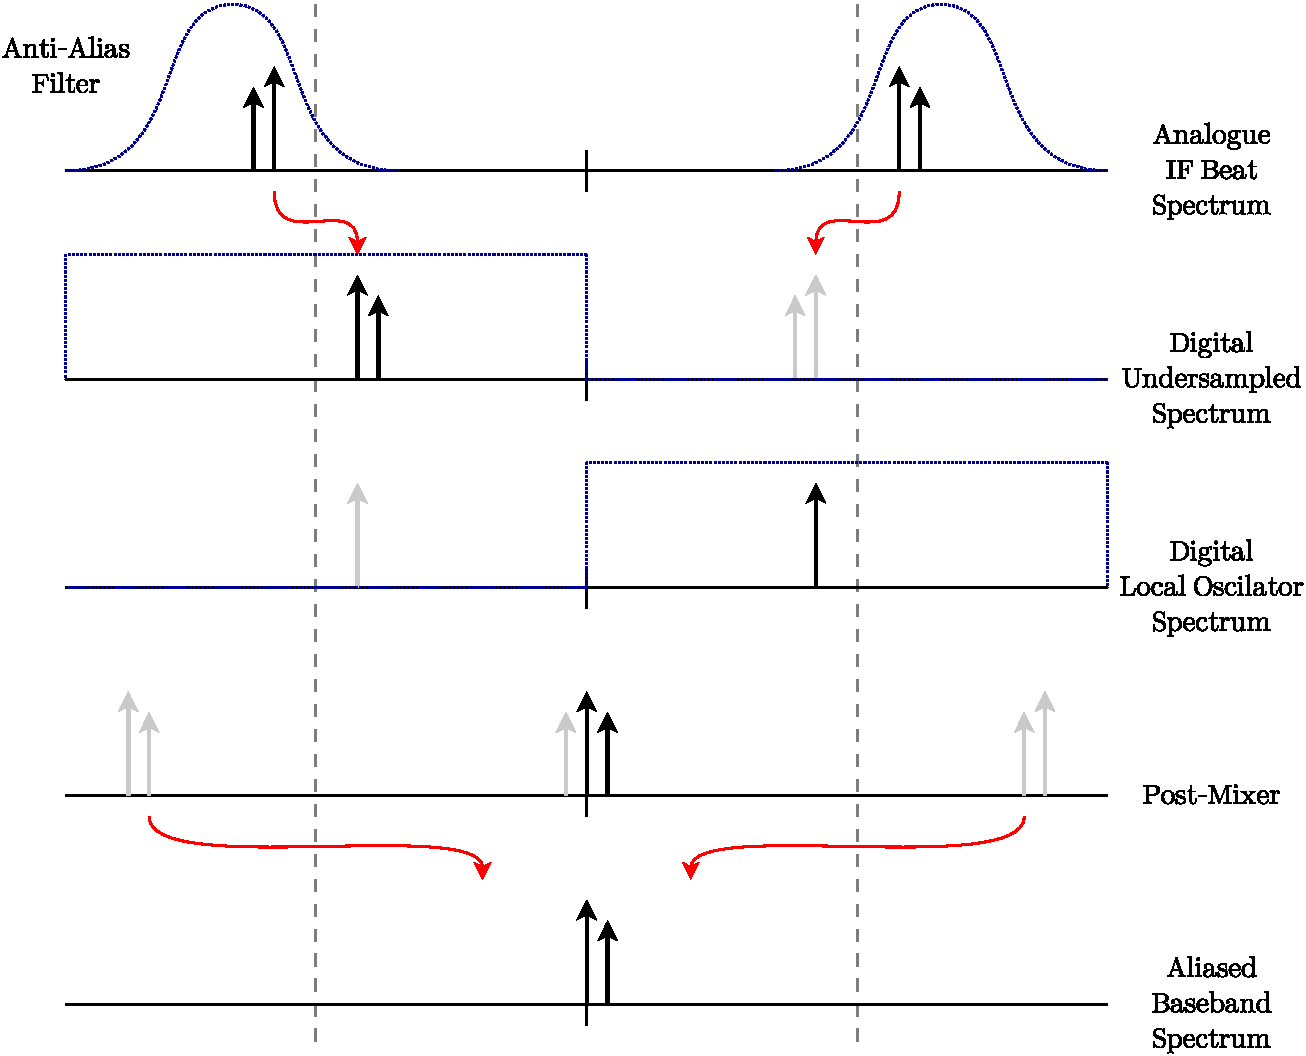
\includegraphics[width=\textwidth]{images/anti_alias_down_conversion}
        \caption{Down-conversion without aliasing.}
        \label{fig:anti_alias_down_conversion}
    \end{center}
\end{figure}

The final processing step is then to preform integration of range profiles on the real data. Addition of two \SI{15}{\bit} numbers results in a single \SI{}{\bit} growth. Our data is now \SI{16}{\bit} and the PRF has been halved, resulting in a halving of the data rate.

As an additional measure for data rate reduction, the unused portion of the FMCW ramp need not be recorded. In other words, the down-ramp portion of the transmitted waveform (which is necessary to maintain PLL lock) need not be stored. \textbf{[Add diagrams for explanation]}

\newpage
\section{Preliminary Results}
\begin{figure}[h!]
    \begin{center}
        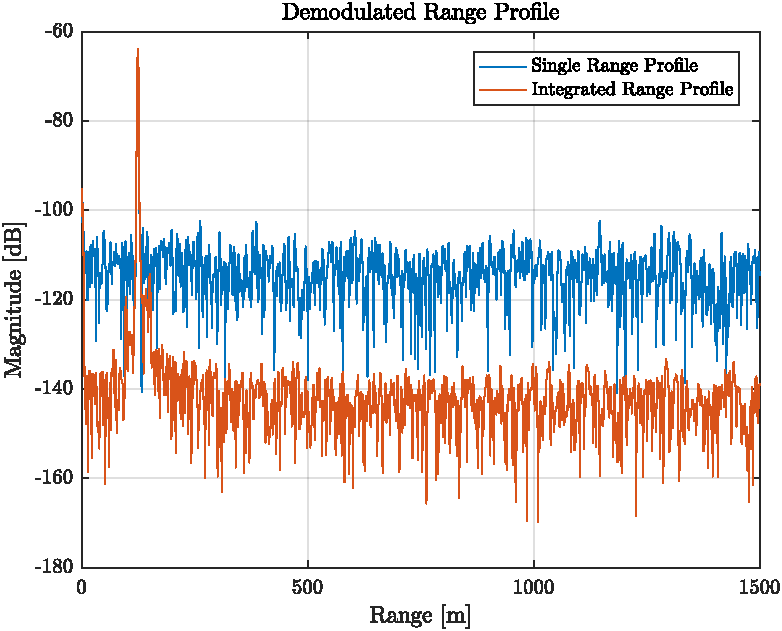
\includegraphics[width=\textwidth]{images/loop_back}
        \caption{Loop-back cable response without the presence of the feed-through return. There is clearly some on-board leakage within the system, manifesting as a peak near DC.}
        \label{fig:loop_back}
    \end{center}
\end{figure}

\begin{figure}[h!]
    \begin{center}
        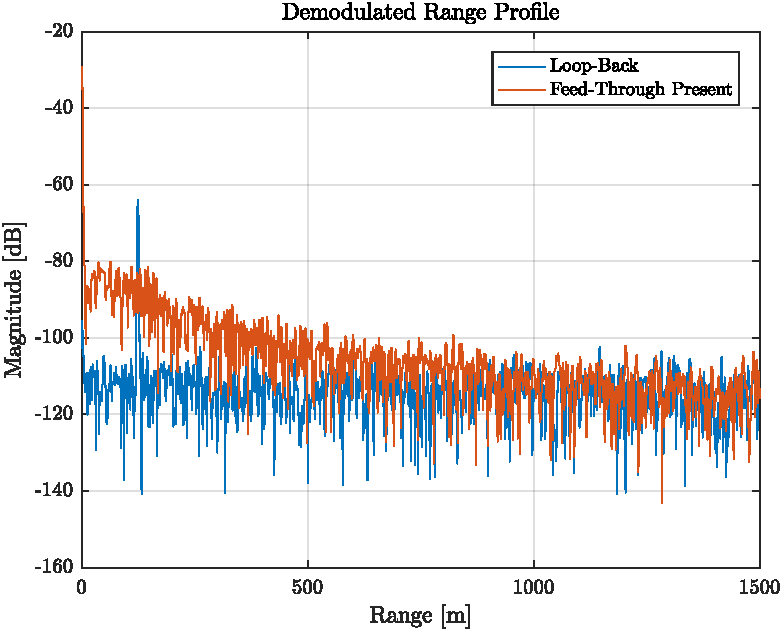
\includegraphics[width=\textwidth]{images/feed_through}
        \caption{Comparison of range profiles for the non-integrated loop-back cable response and the feed-through return. More than \SI{20}{\dB} of SNR is lost to the phase noise of the feed through.}
        \label{fig:feed_through}
    \end{center}
\end{figure}


\end{document}
